\documentclass[a4paper]{article}

\usepackage[francais]{babel}
\usepackage{hyperref}
\usepackage{graphicx}
\usepackage{fontspec}
\usepackage[textwidth=17cm,textheight=27cm]{geometry}

%\setlength{\textwidth}{420 pt} 
%\usepackage{amsmath}
%\usepackage{listings}
%\usepackage{moreverb}
%\usepackage{color}
%\usepackage[colorinlistoftodos]{todonotes}
%\usepackage[labelformat=empty]{caption}

\title{Systèmes multi-agents : la bille, le poisson et l'avatar}

\author{Matthieu CARON - Alexandre MOEVI}

\date{\today}

\begin{document}
\maketitle

\section{Architecture et utilisation}

\subsection{UMLUL}
\url{http://modeling-languages.com/uml-tools/#python}

\subsection{Usage}

\$PYTHONPATH, python3, modifier les paramètres dans MainXXX.py, etc.
\section{Simulations}

\subsection{Tube à particules}

La première simulation, le paquetage \texttt{particules}, reproduit le comportement de billes (ou particules) dans un espace. Cet espace peut torique ou non ; s'il ne l'est pas, les particules rebondissent contre les murs. Les particules rebondissent également en collision.

\medskip
La classe \texttt{Bille} hérite la classe \texttt{Agent} du paquetage \texttt{core}. L'agent \texttt{Bille} connaît son environnement, sa position (entiers \texttt{x} et \texttt{y}) et sa direction (vecteur à 2 dimensions \texttt{[a, b]}).

\medskip
La stratégie d'une particule est la suivante :
\begin{itemize}
\item Dans la méthode \texttt{nextPos()}, la particule calcule sa prochaine possible destination en fonction de l'espace torique (apparition de \og l'autre côté \fg{} de l'écran) ou non (rebond).
\item Dans \texttt{decide()}, la particule regarde sa prochaine destination. Si la voie est libre, elle se prépare à se déplacer (\texttt{particule.bougera = True}). Sinon ça veut dire qu'elle essaye de se rendre dans une case occupée par une autre particule : c'est une collision.
\item Dans \texttt{update()}, si la particule peut bouger, elle se met à sa nouvelle position en laissant libre son ancienne place et l'environnement se met à jour.
\end{itemize}

\medskip
Dans le cas d'une collision (\texttt{particule1.collision(particule2)}), la bille \og incidente \fg{}, c'est-à-dire celle qui essaye d'aller dans une case déjà occupée, échange sa direction avec l'autre particule. Il a été décidé que la bille incidente ne se déplace pas pendant le tick de collision, malgré sa nouvelle direction.
 
\begin{figure}[!h]
\centering
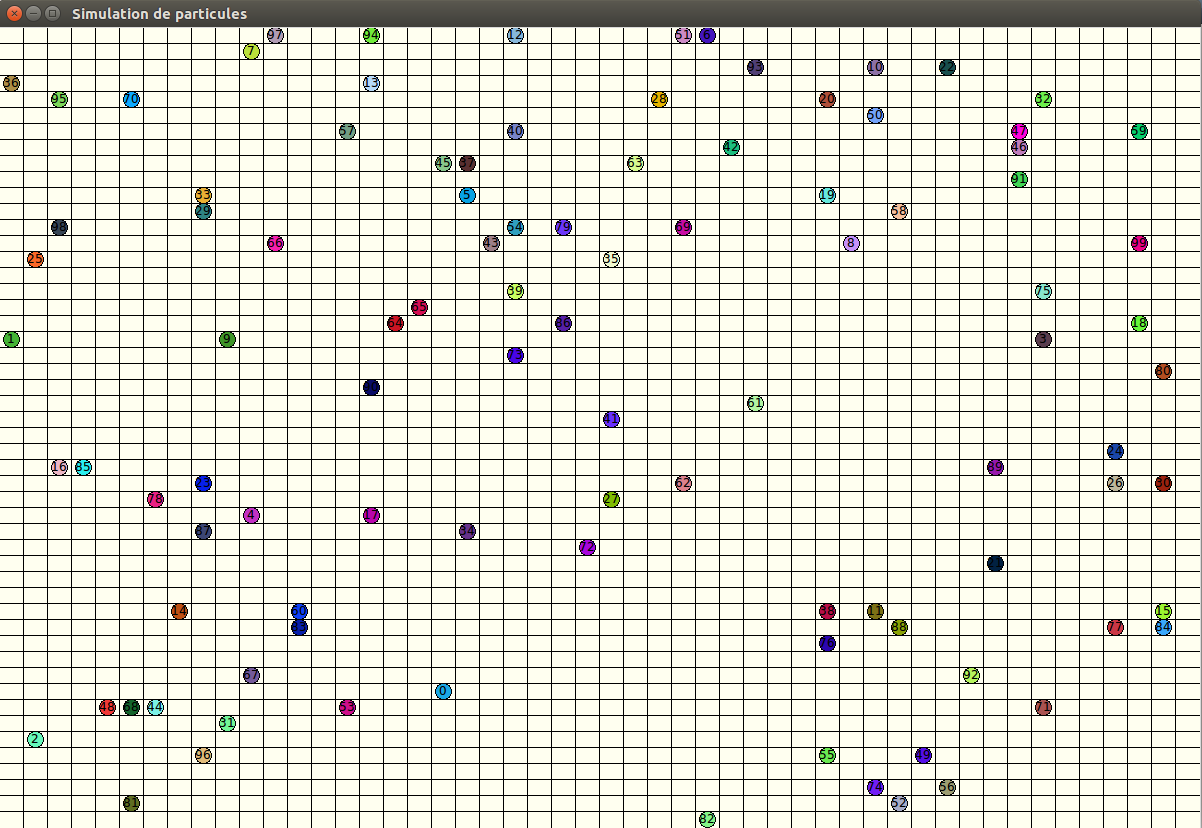
\includegraphics[height=7cm]{particules.png}
\caption{Fenêtre d'exécution du programme \texttt{MainBille}. Les billes sont assignées d'une couleur aléatoire et d'un identifiant pour faciliter leur suivi.}
\end{figure}
\subsection{Poissons et requins dans le golfe (du Bénin)}
La deuxième simulation concerne le paquetage \texttt{wator}. Elle a pour but de voir comment des poissons (les agents \texttt{Fish} dans notre simulation) et des requins (agents \texttt{Shark}) cohabitent dans une zone. 

\medskip
Un agent \texttt{Fish} se déplace de façon aléatoire et se reproduit tous les \texttt{fishBreedTime} ticks. Pour se reproduire, le poisson doit se déplacer et donne naissance à un autre poisson sur la case où il était précédemment.

\medskip
Un \texttt{Shark} est affamé, il a \texttt{dontStarve} ticks pour manger un \texttt{Fish}. S'il n'y arrive pas à temps, il meurt. À l'instar du poisson, il peut se reproduire tous les \texttt{sharkBreedTime} et donne naissance à un nouveau requin sur la case qu'il occupait avant.

\medskip
Comme pour l'agent \texttt{Bille} de la simulation précédente, les agents \texttt{Fish} et \texttt{Shark} ont conscience de leur environnement et connaissent leur coordonnées dans l'espace.

\medskip
Avec ces paramètres, le but est de trouver d'atteindre une situation d'équilibre. On veut éviter une pénurie de poissons (plus de poissons = mort des requins affamés = zone vierge de tout animal) et une absence de requins (les poissons vont se reproduire jusqu'à remplir entièrement la zone).

\medskip
La stratégie d'une 


 
\begin{figure}[!h]
\centering
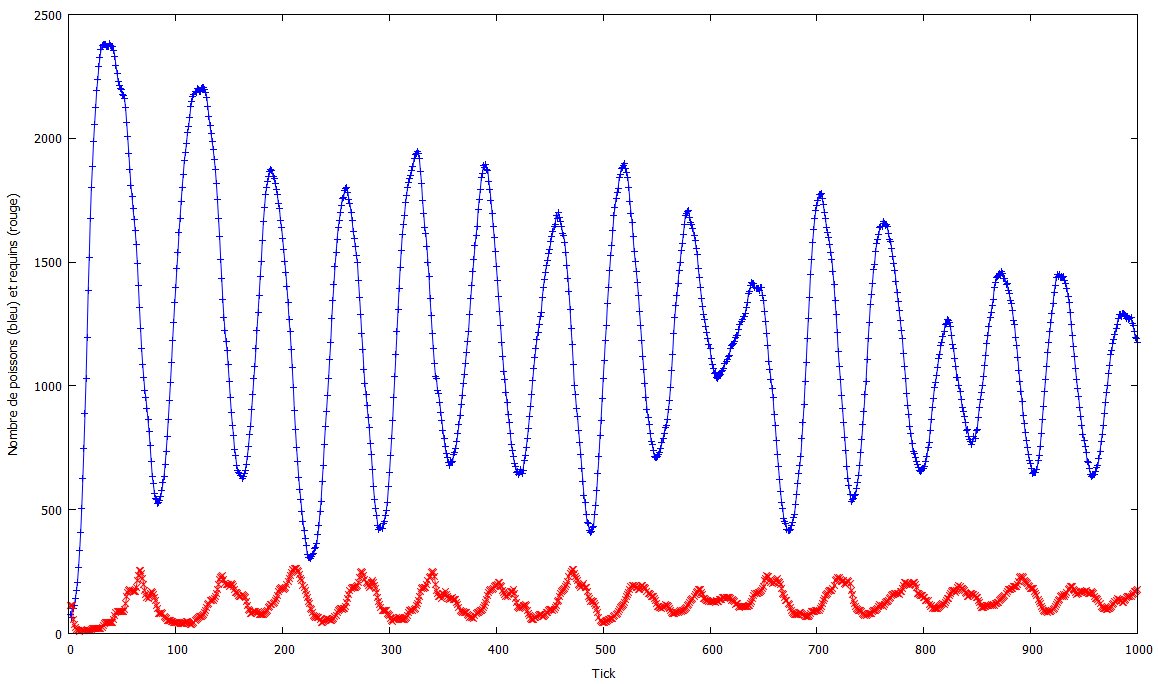
\includegraphics[height=7cm]{1000tours.png}
\caption{Courbes de population.}
\end{figure}

WHY
\subsection{Pac-Man}

\end{document}